\begin{figure}[h!]
\begin{center}
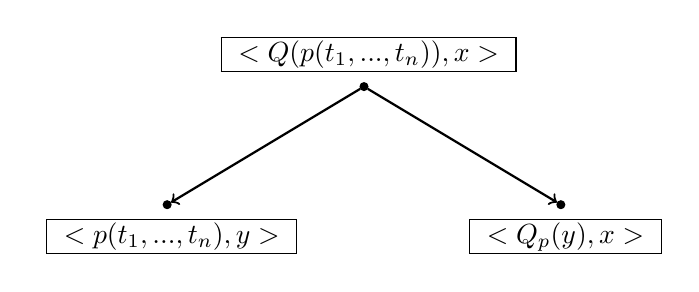
\begin{tikzpicture}[yscale=-1,
place/.style={circle,draw=black, fill=black, inner sep=0pt, 
              minimum size=1mm}]

  \node[place] (1st) at (2.5, 0) [label=above: { 
             \begin{tabular}{|l|}
               \hline
               $<Q(p(t_1,...,t_n)),x>$\\
               \hline
             \end{tabular} }
] {};
	\node[place] (2nd) at (0, 1.5) [label=below: {
              \begin{tabular}{|l|}
                \hline
                 $<p(t_1,...,t_n),y>$ \\
                \hline
              \end{tabular} }
] {};

        \node[place] (3rd) at (5, 1.5) [label=below: {
              \begin{tabular}{|l|}
               \hline
              $<Q_p(y),x>$ \\
               \hline
              \end{tabular} }
] {}; 

	\draw[->, thick] (1st) -- (2nd);
        \draw[->, thick] (1st) -- (3rd);
\end{tikzpicture}
\end{center}
\caption{Finalize the value}
\label{fig:Finalizing}   
\end{figure}